\documentclass{article}
\usepackage[utf8]{inputenc}
\usepackage{listings}
\usepackage{color} %red, green, blue, yellow, cyan, magenta, black, white
\usepackage{graphicx}
\definecolor{mygreen}{RGB}{28,172,0} % color values Red, Green, Blue
\definecolor{mylilas}{RGB}{170,55,241}
\usepackage[margin=0.5in]{geometry}
\usepackage{float}

\lstset{language=Matlab,%
    %basicstyle=\color{red},
    breaklines=true,%
    morekeywords={matlab2tikz},
    keywordstyle=\color{blue},%
    morekeywords=[2]{1}, keywordstyle=[2]{\color{black}},
    identifierstyle=\color{black},%
    stringstyle=\color{mylilas},
    commentstyle=\color{mygreen},%
    tabsize=2,
    showstringspaces=false,%without this there will be a symbol in the places where there is a space
    numbers=left,%
    numberstyle={\tiny \color{black}},% size of the numbers
    numbersep=9pt, % this defines how far the numbers are from the text
    emph=[1]{for,end,break},emphstyle=[1]\color{red}, %some words to emphasise
    %emph=[2]{word1,word2}, emphstyle=[2]{style},    
    literate={~} {$\sim$}{1}
}

\title{Pattern Recognition Assignment 1}
\author{James Jackson}
\date{November 2015}

\begin{document}

\maketitle

\section*{Question 1}
\subsection*{Part A}
\lstinputlisting{ass2Code/assignment2_1a.m}
\begin{figure}[H]
\centering
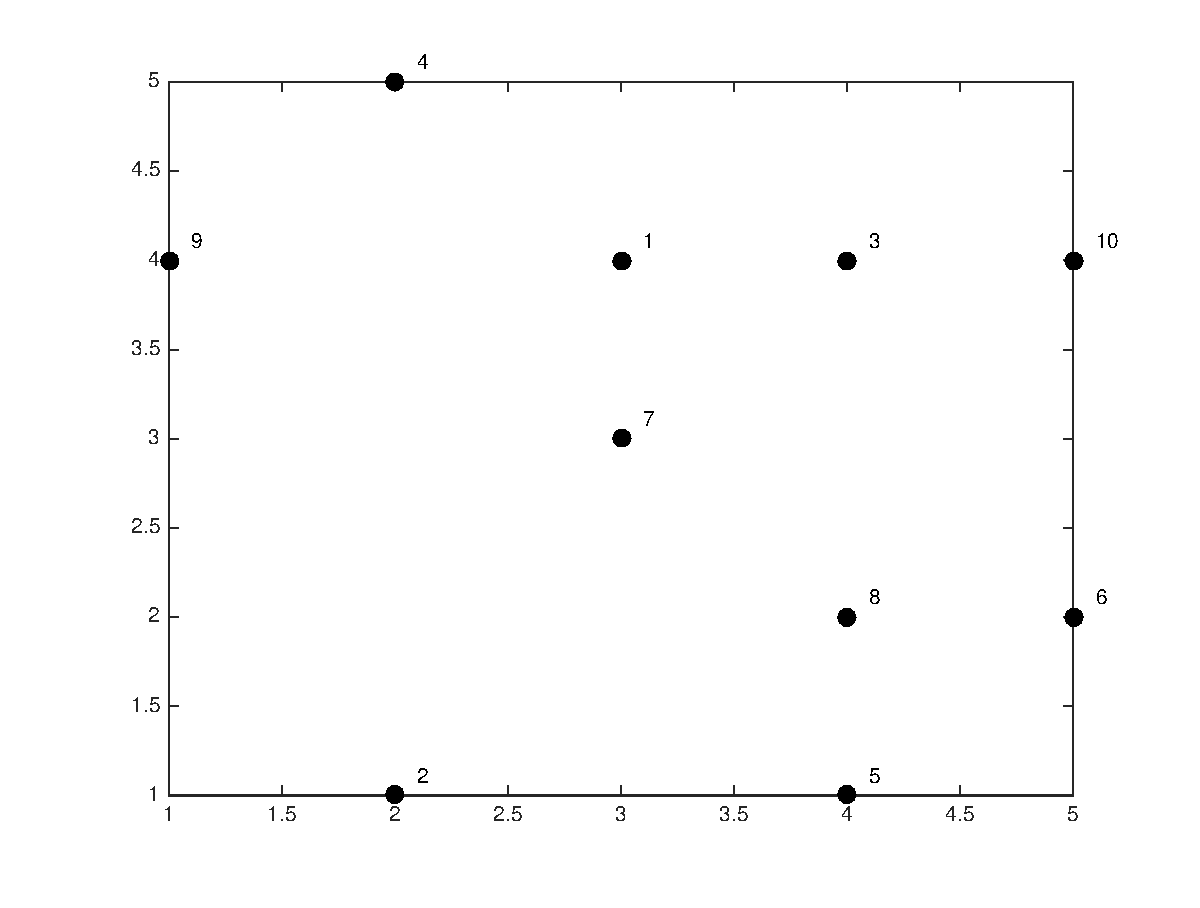
\includegraphics[width=4in]{ass2Code/1a.eps}
\caption{Random plots generated by Question 1 part A}
\end{figure}
\pagebreak
\subsection*{Part B}
\lstinputlisting{ass2Code/assignment2_1b.m}
\textbf{Output}
\begin{lstlisting}
     0    10     1     2    10     8     1     5     4     4
    10     0    13    16     4    10     5     5    10    18
     1    13     0     5     9     5     2     4     9     1
     2    16     5     0    20    18     5    13     2    10
    10     4     9    20     0     2     5     1    18    10
     8    10     5    18     2     0     5     1    20     4
     1     5     2     5     5     5     0     2     5     5
     5     5     4    13     1     1     2     0    13     5
     4    10     9     2    18    20     5    13     0    16
     4    18     1    10    10     4     5     5    16     0
\end{lstlisting}
\subsection*{Part C}
\lstinputlisting{ass2Code/assignment2_1c.m}
\begin{figure}[H]
\centering
\includegraphics[width=4in]{ass2Code/1c.eps}
\caption{Clustered points}
\end{figure}
\pagebreak
\subsection*{Part D}
\textbf{Kruskals Minimum Spanning Tree with Step Return}
\lstinputlisting{kruskals_mst_with_steps.m}
\textbf{Using the above function we now output the steps to the console}
\lstinputlisting{ass2Code/assignment2_1d.m}
\pagebreak
\textbf{Output}
\begin{lstlisting}
Step   1 J =   0, #Cl  10: ( 1 ) ( 2 ) ( 3 ) ( 4 ) ( 5 ) ( 6 ) ( 7 ) ( 8 ) ( 9 ) ( 10 )
Step   2 J =   1, #Cl   9: ( 2 ) ( 1 3 ) ( 4 ) ( 5 ) ( 6 ) ( 7 ) ( 8 ) ( 9 ) ( 10 )
Step   3 J =   1, #Cl   8: ( 2 ) ( 4 ) ( 5 ) ( 6 ) ( 1 3 7 ) ( 8 ) ( 9 ) ( 10 )
Step   4 J =   1, #Cl   7: ( 2 ) ( 4 ) ( 5 ) ( 6 ) ( 8 ) ( 9 ) ( 1 3 7 10 )
Step   5 J =   1, #Cl   6: ( 2 ) ( 4 ) ( 6 ) ( 5 8 ) ( 9 ) ( 1 3 7 10 )
Step   6 J =   1, #Cl   5: ( 2 ) ( 4 ) ( 5 6 8 ) ( 9 ) ( 1 3 7 10 )
Step   7 J =   2, #Cl   4: ( 2 ) ( 1 3 4 7 10 ) ( 5 6 8 ) ( 9 )
Step   8 J =   2, #Cl   3: ( 2 ) ( 5 6 8 ) ( 1 3 4 7 9 10 )
\end{lstlisting}

\subsection*{Part E}
\lstinputlisting{ass2Code/assignment2_1e.m}
\textbf{Output}
\begin{lstlisting}
Suggested Clustering
Step   6 J =   1, #Cl   5: ( 2 ) ( 4 ) ( 5 6 8 ) ( 9 ) ( 1 3 7 10 )
\end{lstlisting}

\section*{Question 2}
\subsection*{Part A}
\lstinputlisting{ass2Code/assignment2_2a.m}
\textbf{Output}
\begin{figure}[H]
\centering
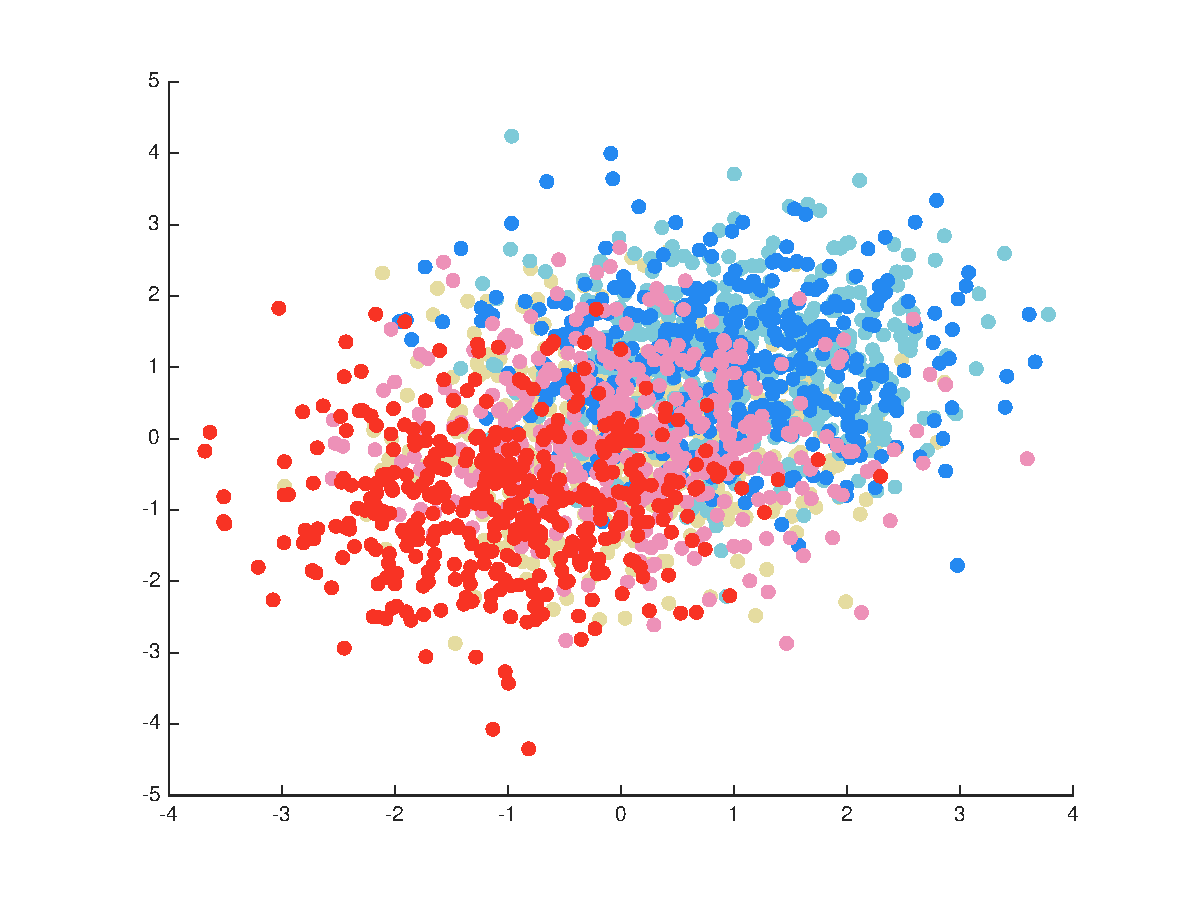
\includegraphics[width=4in]{ass2Code/2a.eps}
\caption{Data plotted from 2A}
\end{figure}

\subsection*{Part B}
\lstinputlisting{ass2Code/assignment2_2b.m}
\textbf{Output}
\begin{figure}[H]
\centering
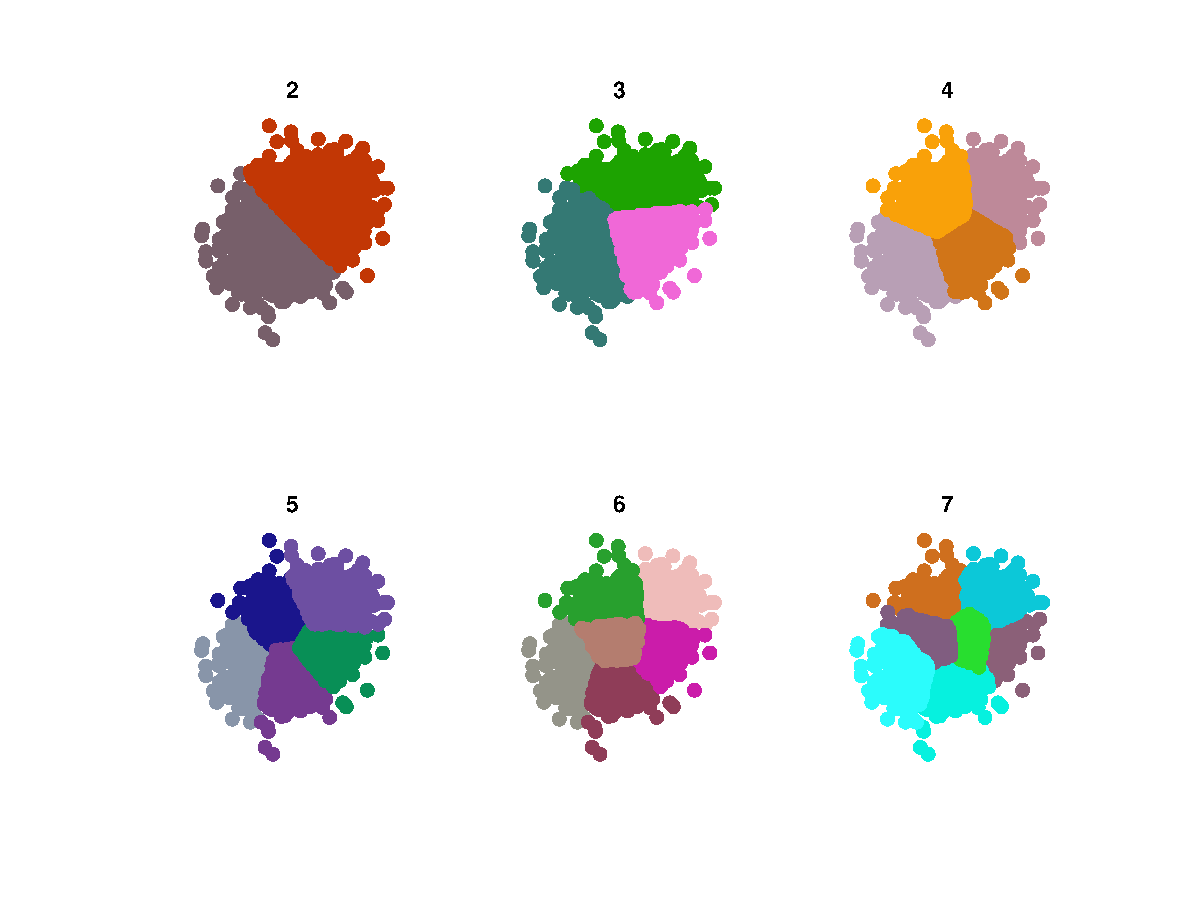
\includegraphics[width=4in]{ass2Code/2b.eps}
\caption{Clustered forms of data from 2a}
\end{figure}
\pagebreak
\section*{Question 3}
\subsection*{Part A}
\lstinputlisting{ass2Code/assignment2_3a.m}
\subsection*{Part B}
\lstinputlisting{ass2Code/assignment2_3b.m}

\textbf{Output}
\begin{lstlisting}
Feature		J
===			===
488			149.10 
489			148.48 
462			141.63 
461			139.66 
516			138.49 
515			130.65 
490			122.05 
463			119.22 
517			117.49 
487			117.24 
\end{lstlisting}
\pagebreak
\subsection*{Part C}
\lstinputlisting{ass2Code/assignment2_3c.m}
\textbf{Output}
\begin{figure}[H]
\centering
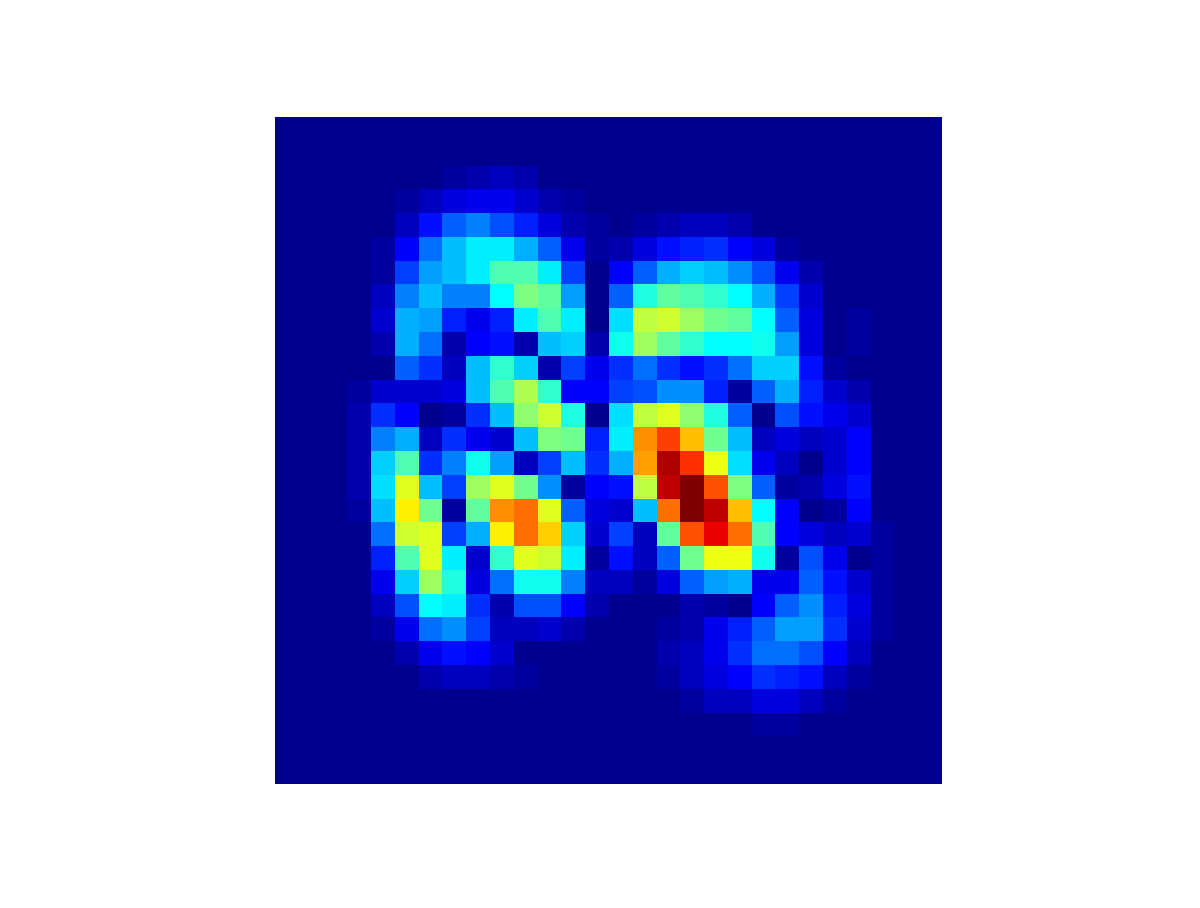
\includegraphics[width=4in]{ass2Code/3c.eps}
\caption{Image representation of criteron values}
\end{figure}

\subsection*{Part D}
\lstinputlisting{ass2Code/assignment2_3d.m}
\textbf{Output}
\begin{lstlisting}
badF =
	235
\end{lstlisting}
\begin{figure}[H]
\centering
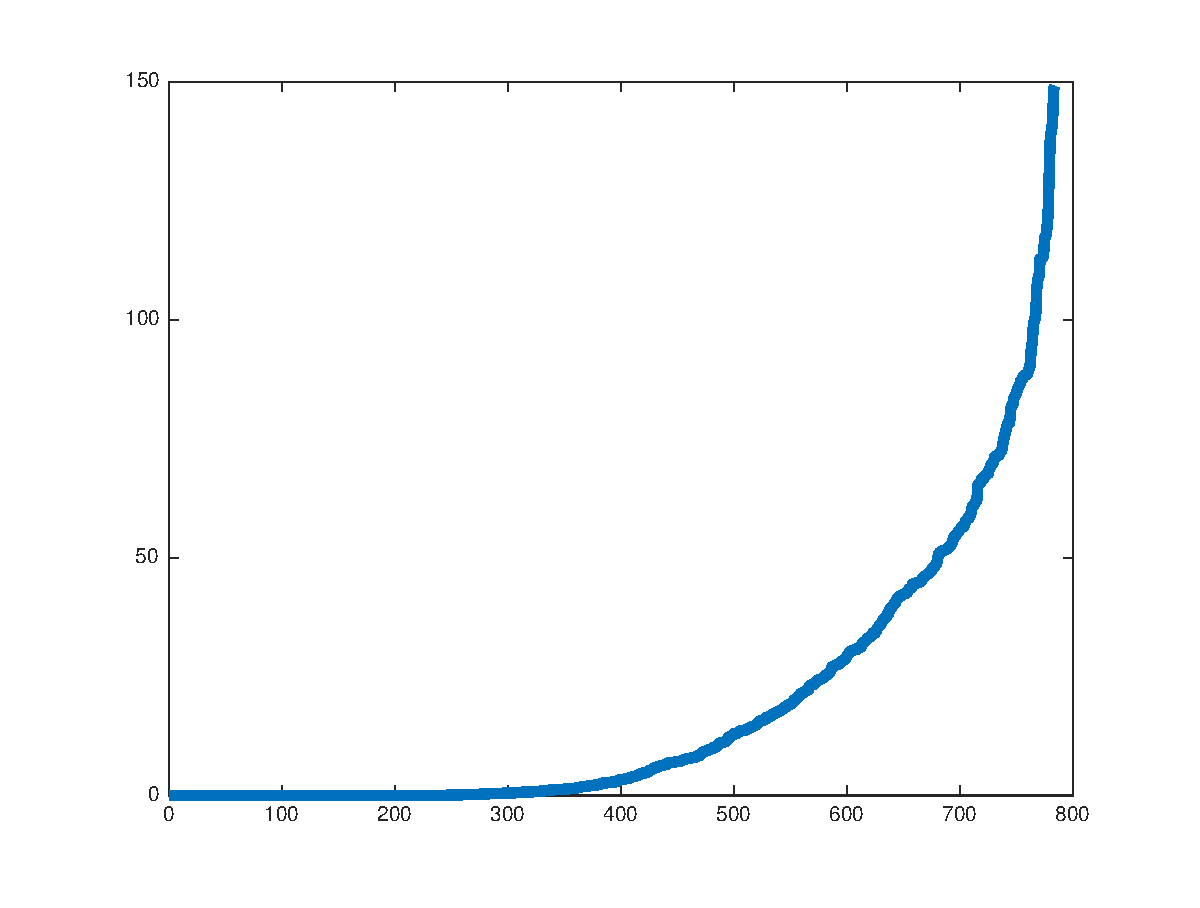
\includegraphics[width=4in]{ass2Code/3d.eps}
\caption{Plot of J values}
\end{figure}

\subsection*{Part E}
\lstinputlisting{ass2Code/assignment2_3e.m}
\begin{figure}[H]
\centering
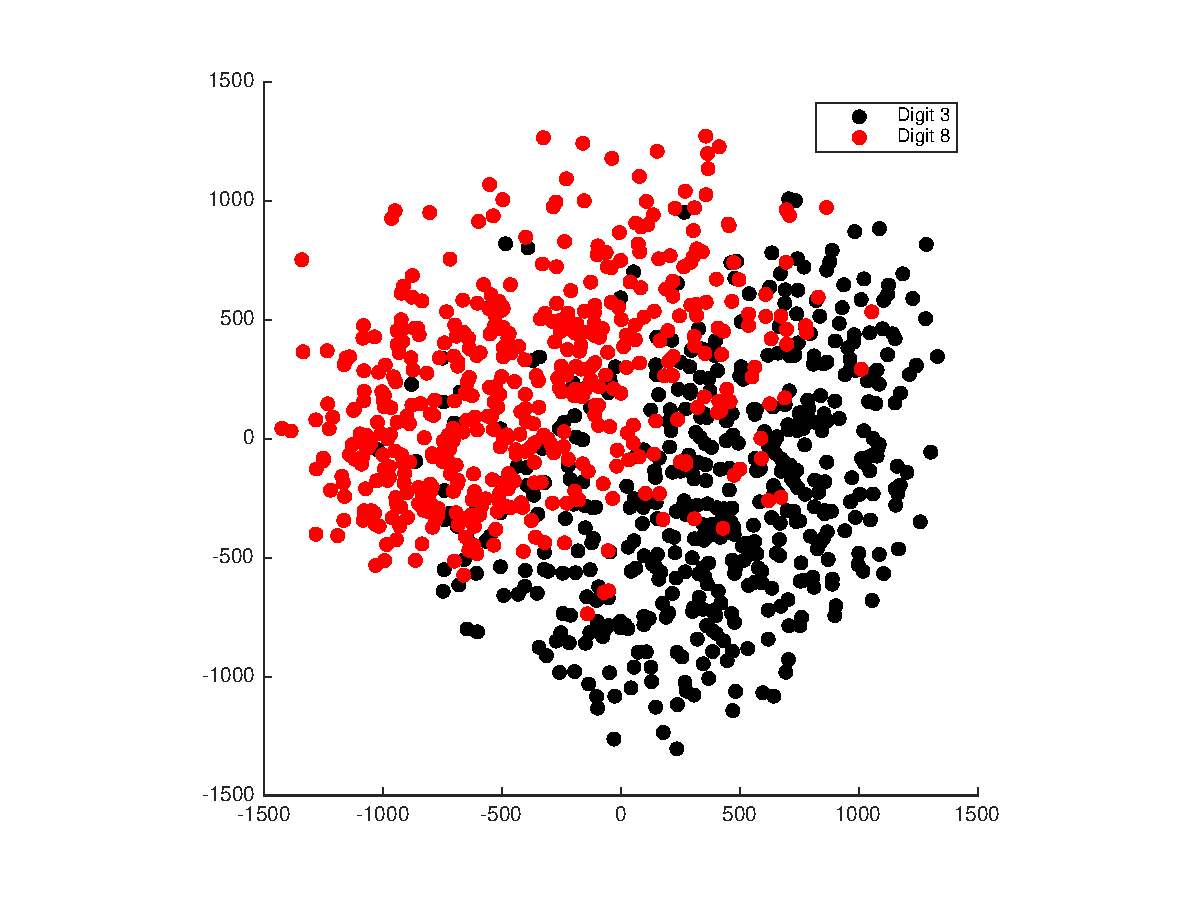
\includegraphics[width=4in]{ass2Code/3e.eps}
\caption{Plot of first two PC}
\end{figure}

\pagebreak
\subsection*{Part F}
\lstinputlisting{ass2Code/assignment2_3f.m}
\textbf{Output}
\begin{lstlisting}
rE1 =
	0.1421
rE2 =
	0.1285
\end{lstlisting}

The resubstitution errors between these two feature representations is very similar. In this case, selecting the top 8 features gives a marginally better result. Increasing the number of features selected continues the trend but closes the gap, for example. If we select the to 16 features and take the first 16 componentes our results are:
\begin{lstlisting}
rE1 =
	0.1181
rE2 =
	0.1202
\end{lstlisting}

When we reduce the number to 4 there is still marginal difference between the two methods but PC performs better.
\begin{lstlisting}
rE1 =
	0.1755
rE2 =
	0.1526
\end{lstlisting}

Principal component analysis analyses the variance between features and returns the highest to lowest in terms of this variance. For our 2D dataset the variance between features is the distance between them so our univariant feature selection is essentially applying the same metohd for ranking features which leads to the very similar outputs.

\section*{Question 4}

\lstinputlisting{ass2Code/perceptron.m}

\lstinputlisting{ass2Code/assignment2_4.m}
\textbf{Output}
\begin{figure}[H]
\centering
\includegraphics[width=4in]{ass2Code/4a.eps}
\caption{Perceptron Learning Rate 0.1}
\end{figure}
\begin{figure}[H]
\centering
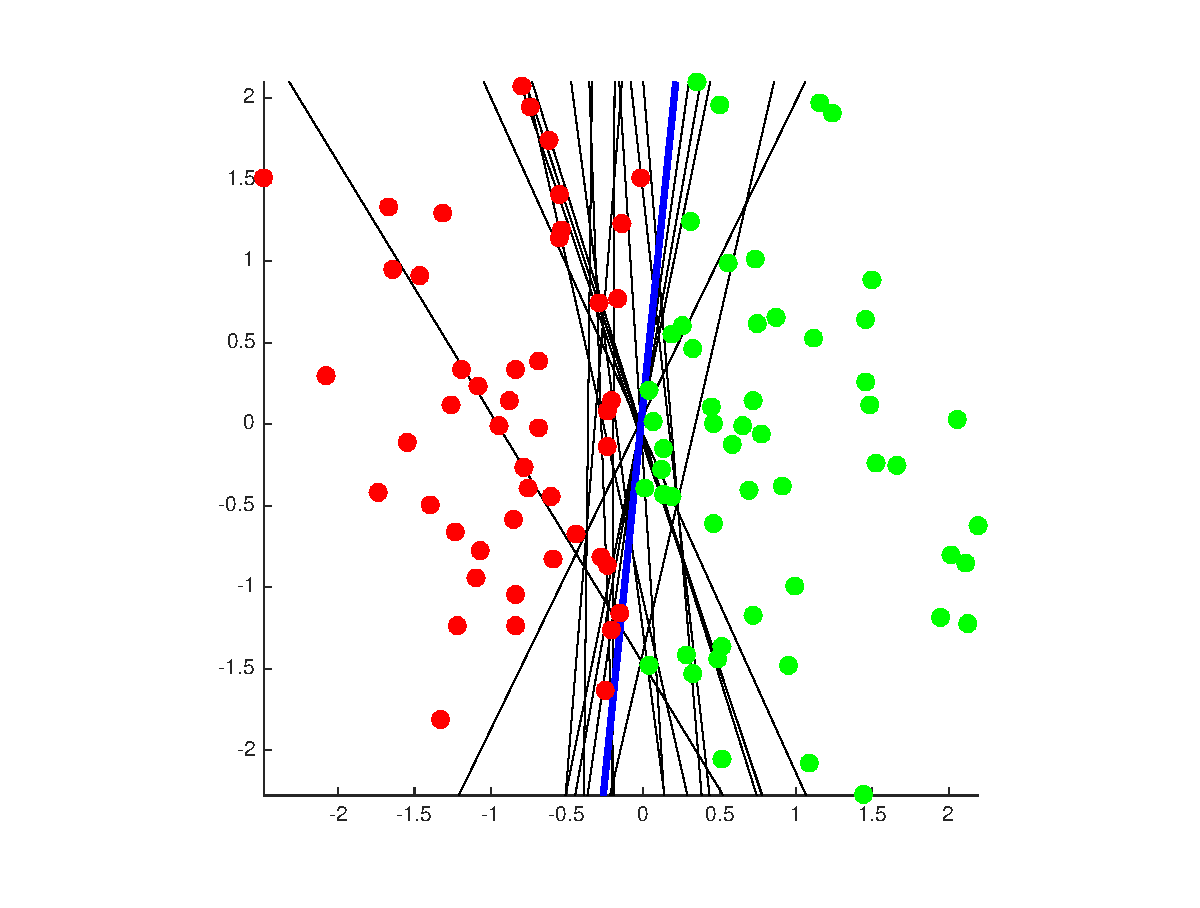
\includegraphics[width=4in]{ass2Code/4b.eps}
\caption{Perceptron Learning Rate 0.8}
\end{figure}

With a lower learning rate, the weights are updated in smaller increments. In the above case this has meant for much more iterations before converging, the heigher learning rate required fewer iterations. However a higher learning rate means a larger movement in the boundary so. This large movement could `overshoot' the required boundary and lead to more iteratoins.
 
As a further test both learning rates were tested 100 times and the epochs counted giving the following means as a result.

\begin{lstlisting}
lowLR =
	3.1100
highLR =
	4.9000
\end{lstlisting}

While far from exhaustive, this test implies that a higher learning rate is less efficient than a smaller learning rate from this data.

\section*{Question 5}

\lstinputlisting{ass2Code/assignment2_5.m}
\begin{figure}[H]
\centering
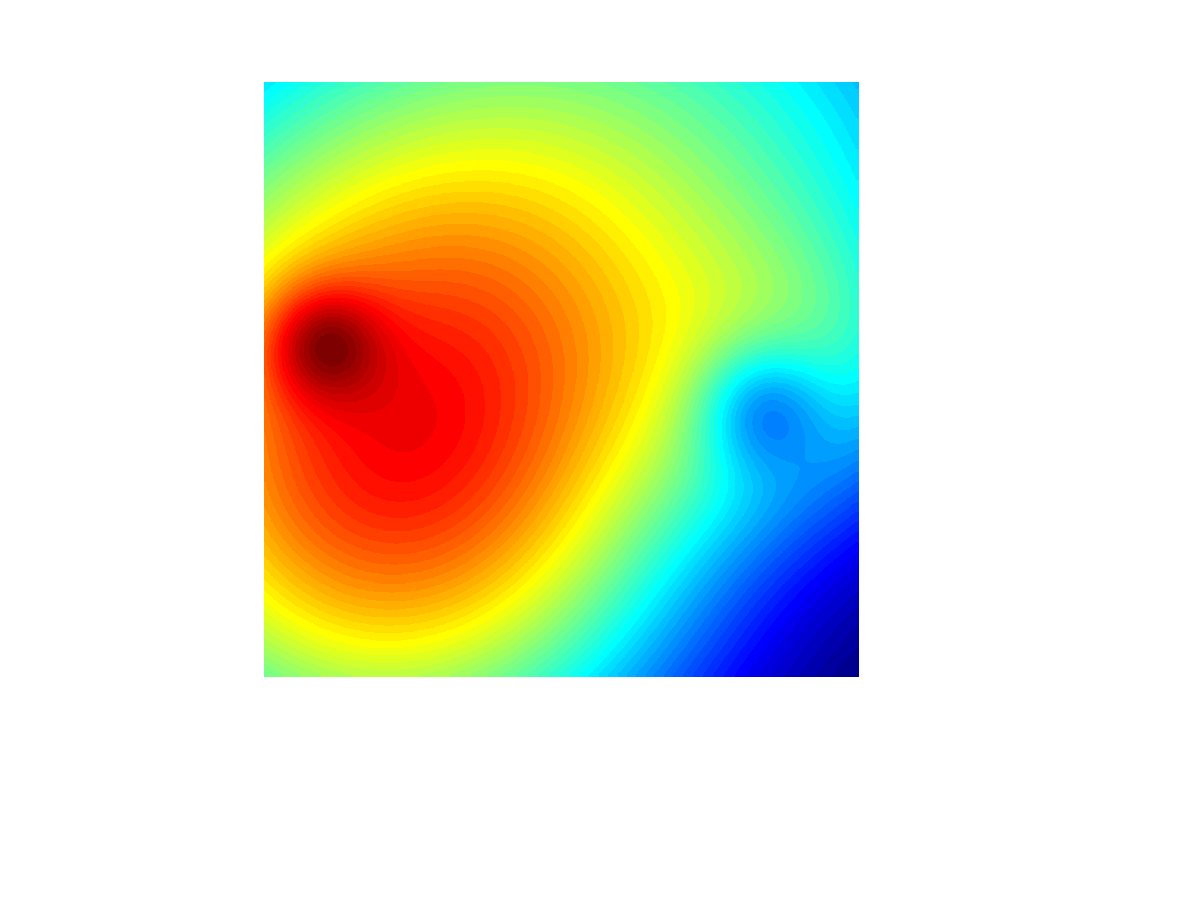
\includegraphics[width=4in]{ass2Code/5.eps}
\caption{Visualised RBF Function}
\end{figure}
\begin{figure}[H]
\centering
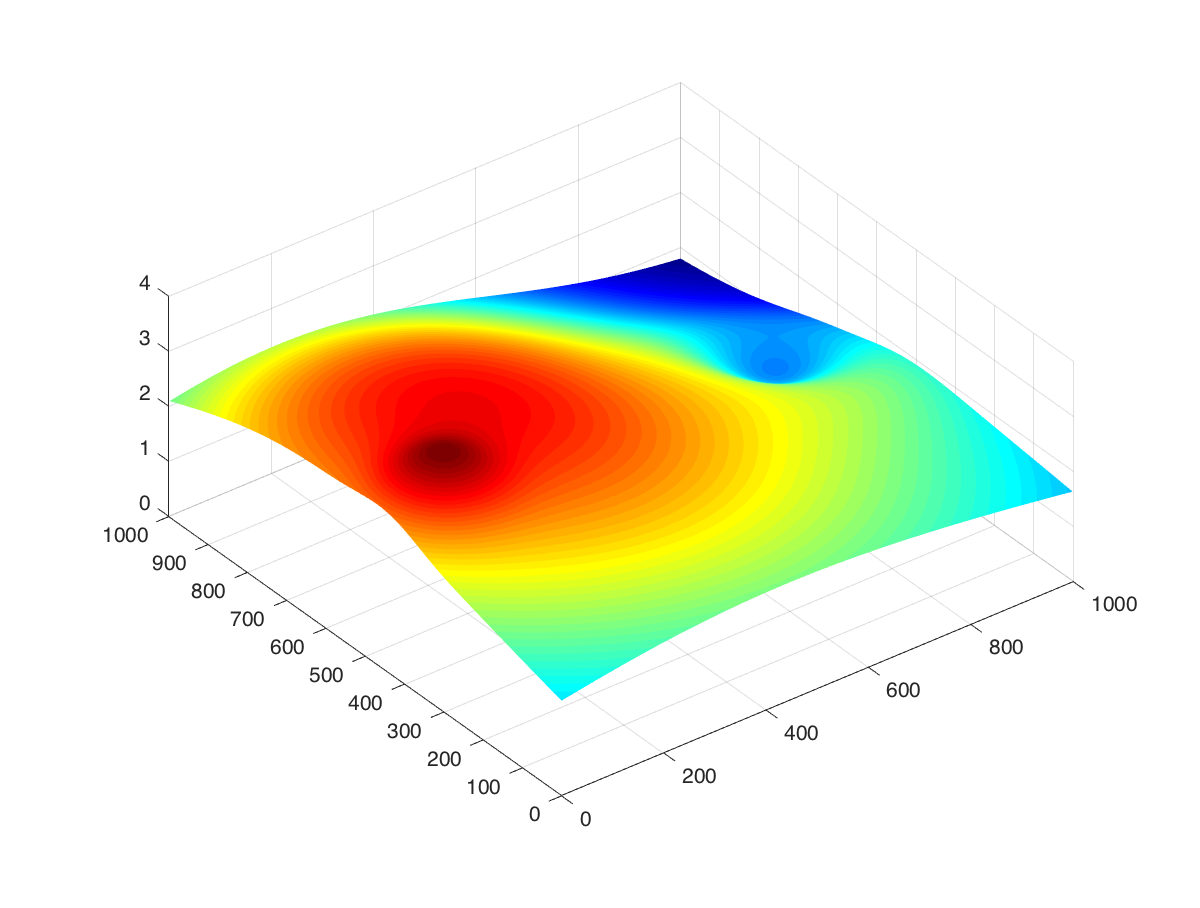
\includegraphics[width=4in]{ass2Code/5b.eps}
\caption{Visualised RBF Function Surface plot}
\end{figure}
Used a surface plot to further visualise the output of the funtion.

\end{document}